\definecolor{mygrey}{rgb}{0.95, 0.95, 0.92}

\section{Bài 1}
\subsection{Cấu trúc dữ liệu biểu diễn}
\subsubsection{Danh sách kề}
Một cách để biểu diễn đồ thị không có cạnh song song là liệt kê tất cả các cạnh của đồ thị này. Một cách khác để biểu diễn một đồ thị không có cạnh song song là sử dụng danh sách kề, trong đó xác định các đỉnh kề với mỗi đỉnh của đồ thị.

\textbf{Ví dụ 1:}
Sử dụng danh sách kề để mô tả đơn đồ thị sau đây:
\begin{figure}[H] % places figure environment here   
    \centering % Centers Graphic
    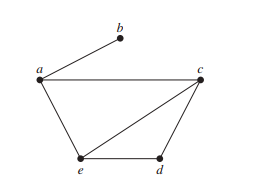
\includegraphics[width=0.4\textwidth]{assets/pic1.png} 
\end{figure}

\textbf{Cách giải:} Bảng dưới đây liệt kê các đỉnh kề với mỗi đỉnh của đồ thị:

\begin{figure}[H] % places figure environment here   
    \centering % Centers Graphic
    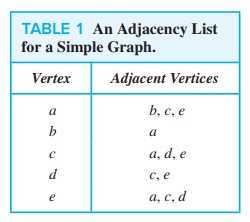
\includegraphics[width=0.3\textwidth]{assets/pic2.png} 
    \label{fig:gr_01}
\end{figure}

\textbf{Ví dụ 2:}
Biểu diễn đồ thị có hướng trong Hình sau đây bằng cách liệt kê tất cả các đỉnh cuối của các cạnh bắt đầu tại mỗi đỉnh của đồ thị.
\begin{figure}[H] % places figure environment here   
    \centering % Centers Graphic
    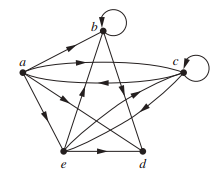
\includegraphics[width=0.4\textwidth]{assets/pic1.1.png} 
\end{figure}

\textbf{Cách giải:} Bảng sau biểu diễn đồ thị có hướng như yêu cầu của đề bài:
\begin{figure}[H] % places figure environment here   
    \centering % Centers Graphic
    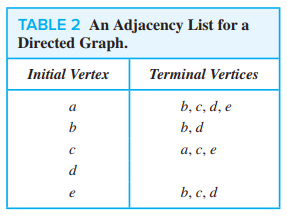
\includegraphics[width=0.3\textwidth]{assets/pic2.1.png} 
    \label{fig:gr_01}
\end{figure}


\subsubsection{Ma trận kề}
Việc thực hiện các thuật toán đồ thị bằng cách biểu diễn đồ thị bằng danh sách các cạnh, hoặc bằng danh sách kề, có thể phức tạp nếu có nhiều cạnh trong đồ thị. Để đơn giản hóa việc tính toán, đồ thị có thể được biểu diễn bằng ma trận. Hai loại ma trận thường dùng để biểu diễn đồ thị sẽ được trình bày ở đây. Một dựa trên sự kề nhau của các đỉnh, và một dựa trên tỷ lệ các đỉnh và cạnh.

Giả sử rằng $G = (V, E)$ là một đơn đồ thị, trong đó $|V| = n$. Giả sử rằng các đỉnh của G được liệt kê tùy ý là $v_1, v_2,…, v_n$. \textbf{Ma trận kề A} (hoặc $A_G$) của G, đối với danh sách các đỉnh này, là ma trận gồm các phần tử 0 và 1, cỡ n x n, với 1 là phàn tử thứ (i,j) nếu $v_i và v_j$ là liền kề, và 0 là mục nhập thứ (i,j) của nó khi hai cạnh tương ứng không liền kề. Nói cách khác, nếu ma trận kề là $A = [a_{ij}$], thì:

$
a_{ij} = \left\{ \begin{array}{lcr}
1 & \text{nếu ${v_i, v_j}$ là một cạnh của G}\\
0 & \text{với các trường hợp còn lại}
\end{array} \right.
$


\textbf{Ví dụ:}
Vẽ đồ thị với ma trận kề sau:

$
\begin{bmatrix}
    0&1&1&0\\
    1&0&0&1\\
    1&0&0&1\\
    0&1&1&0
\end{bmatrix}
$
theo thứ tự các đỉnh a, b, c, d.

\textbf{Cách giải:}
Đồ thị của ma trận kề được thể hiện trong hình sau:

\begin{figure}[H] % places figure environment here   
    \centering % Centers Graphic
    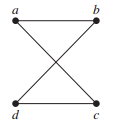
\includegraphics[width=0.2\textwidth]{assets/pic3.png} 
    \label{fig:gr_01}
\end{figure}


Lưu ý rằng ma trận kề của đồ thị dựa trên thứ tự được chọn cho các đỉnh. Do đó, có thể có nhiều nhất là n! các ma trận kề khác nhau cho một đồ thị có n đỉnh, vì có n! các tổ hợp khác nhau của n đỉnh.

Ma trận kề của một đơn đồ thị là ma trận đối xứng, nghĩa là, $a_{ij} = a_{ji}$, bởi vì cả hai mục này là 1 khi $v_i và v_j$ kề nhau, và cả hai đều bằng 0 trong trường hợp ngược lại. Hơn nữa, bởi vì một đơn đồ thị không có khuyên (loop), mỗi phần tử $a_{ij}, i = 1, 2, 3,…, n$, đều bằng 0.

Ma trận kề cũng có thể được sử dụng để biểu diễn đồ thị vô hướng với các khuyên và với các cạnh song song. Khuyên ở đỉnh $v_i$ được biểu diễn bằng 1 ở vị trí thứ (i,i) của ma trận kề. Khi các cạnh song song nối cùng một cặp đỉnh vi và vj, hoặc nhiều khuyên tại cùng một đỉnh, thì ma trận kề không còn là ma trận 0-1 nữa, vì phần tử thứ (i,j) của ma trận này bằng số cạnh được nối với ${v_i, v_j}$. Tất cả các đồ thị vô hướng, bao gồm cả đa đồ thị, đều có ma trận kề đối xứng.

\subsubsection{So sánh Danh sách kề và Ma trận kề}
Khi một đơn đồ thị chứa tương đối ít cạnh, hay còn gọi là \textbf{thưa thớt}, thường nên sử dụng danh sách kề hơn là ma trận kề để biểu diễn đồ thị. Ví dụ, nếu mỗi đỉnh có bậc không vượt quá c, trong đó c là hằng số nhỏ hơn n rất nhiều, thì mỗi danh sách kề sẽ chứa c hoặc ít đỉnh hơn. Do đó, không có nhiều hơn $cn$ mục trong tất cả các danh sách gần kề này. Mặt khác, ma trận kề của đồ thị sẽ có $n\sp{2}$ phần tử. Tuy nhiên, lưu ý rằng ma trận kề của một đồ thị thưa là một \textbf{ma trận thưa}, là ma trận có ít phần tử khác 0, và sẽ có các kỹ thuật đặc biệt để biểu diễn và tính toán với ma trận thưa.

Bây giờ, giả sử rằng một đơn đồ thị là đồ thị dày đặc (dense), nghĩa là, giả sử rằng nó chứa nhiều cạnh, chẳng hạn như một đồ thị chứa hơn một nửa tổng số các cạnh có thể có. Trong trường hợp này, sử dụng ma trận kề để biểu diễn đồ thị thường thích hợp hơn việc sử dụng danh sách kề. Để giải thích tại sao, ta so sánh độ phức tạp của việc xác định xem cạnh ${v_i, v_j}$ có tồn tại hay không. Sử dụng ma trận kề, chúng ta có thể xác định xem cạnh này có tồn tại hay không bằng cách kiểm tra phần tử thứ ${i,j}$ trong ma trận. Phần tử này là 1 nếu đồ thị chứa cạnh này và bằng 0 nếu ngược lại. Do đó, chúng ta chỉ cần thực hiện một phép so sánh, đó là so sánh phần tử này với 0, để xác định xem cạnh này có tồn tại hay không. Mặt khác, khi chúng ta sử dụng danh sách kề để biểu diễn đồ thị, chúng ta cần tìm kiếm danh sách các đỉnh kề với $v_i$ hoặc $v_j$ để xác định xem có cạnh này hay không. Điều này có thể yêu cầu $\theta(|V|)$ so sánh trong trường hợp có nhiều cạnh.


\subsubsection{Ma trận liên thuộc (Incidence Matrices)}
Một cách phổ biến khác để biểu diễn đồ thị là sử dụng \textbf{ma trận liên thuộc}. Gọi G = (V, E) là một đồ thị vô hướng. Giả sử rằng $v_1, v_2,…, v_n$ là các đỉnh và $e_1, e_2,…, e_m$ là các cạnh của G. Khi đó ma trận tương ứng của V và E là ma trận $n*m$ $M = [m_{ij}]$ , với

$
m_{ij} = \left\{ \begin{array}{lcr}
1 & \text{khi $e_j$ kề với $v_i$}\\
0 & \text{với các trường hợp còn lại}
\end{array} \right.
$

\textbf{Ví dụ:}
Biểu diễn đồ thị trong hình dưới đây bằng một ma trận liên thuộc:

\begin{figure}[H]    
    \centering % Centers Graphic
    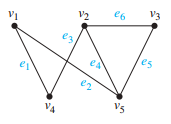
\includegraphics[width=0.2\textwidth]{assets/pic4.png}
    \caption{Đồ thị vô hướng}
    %\label{fig:gr_01}
\end{figure}


\textbf{Cách giải:} Ma trận liên thuộc là:

\begin{figure}[H]    
    \centering % Centers Graphic
    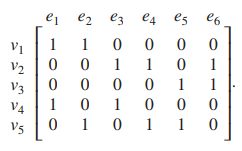
\includegraphics[width=0.2\textwidth]{assets/pic5.png}
    %\label{fig:gr_01}
\end{figure}

Ma trận liên thuộc cũng có thể được sử dụng để biểu diễn cạnh song song và khuyên. Các cạnh song song được biểu diễn trong ma trận liên thuộc bằng cách sử dụng các cột có các phần tử giống nhau, bởi vì các cạnh này kề với cùng một cặp đỉnh. Các khuyên được biểu diễn bằng cách sử dụng một cột có chính xác một phần tử bằng 1, tương ứng với đỉnh kề với khuyên này.

\subsection{Mô hình và ứng dụng của đồ thị trong bài toán thực tiễn}

\subsubsection{Mạng xã hội}

Đồ thị được sử dụng rộng rãi để mô hình hóa cấu trúc xã hội dựa trên các loại mối quan hệ khác nhau giữa người hoặc nhóm người. Các cấu trúc xã hội này và biểu đồ đại diện cho chúng được gọi là \textbf{mạng xã hội}. Trong các mô hình đồ thị này, các cá nhân hoặc tổ chức được biểu diễn bằng các đỉnh; mối quan hệ giữa các cá nhân hoặc tổ chức được thể hiện bằng các cạnh. Nghiên cứu về mạng xã hội là một lĩnh vực đa ngành cực kỳ năng động, và nhiều loại mối quan hệ khác nhau giữa mọi người đã được nghiên cứu bằng cách sử dụng chúng. Trong phần này, ta sẽ tìm hiểu một số mạng xã hội phổ biến nhất được nghiên cứu.

\textbf{Ví dụ 1: Đồ thị tình bạn và mối quan hệ}
Chúng ta có thể sử dụng một biểu đồ đơn giản để biểu diễn liệu hai người có biết nhau hay không, tức là họ có quen biết hay là bạn bè (trong thế giới thực hoặc trong thế giới ảo thông qua một trang mạng xã hội, ví dụ như Facebook). Mỗi người trong một nhóm người cụ thể được biểu diễn bằng một đỉnh. Một cạnh vô hướng được sử dụng để kết nối hai người khi những người này biết nhau, khi chúng ta chỉ quan tâm đến mối quan hệ quen biết, hoặc liệu họ có phải là bạn bè hay không. Không có các cạnh song song và thường không có khuyên nào được sử dụng. (Nếu muốn bao gồm khái niệm về việc tự nhận thức về bản thân (self-knowledge), ta sẽ dùng thêm các vòng lặp). Một đồ thị nhỏ về mối quan hệ quen biết được thể hiện trong dưới đây.

\begin{figure}[H] % places figure environment here   
    \centering % Centers Graphic
    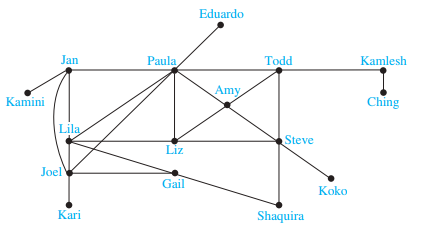
\includegraphics[width=0.4\textwidth]{assets/pic6.png} 
    \caption{Đồ thị tình bạn và mối quan hệ} % Creates caption underneath graph
\end{figure}

\textbf{Ví dụ 2: Đồ thị ảnh hưởng}
Trong các nghiên cứu về hành vi của nhóm, người ta quan sát thấy rằng một số người nhất định có thể ảnh hưởng đến suy nghĩ của người khác. Đồ thị có hướng, được gọi là \textbf{đồ thị ảnh hưởng}, có thể được sử dụng để mô hình hóa hành vi này. Mỗi người trong nhóm được biểu diễn bằng một đỉnh. Có một cạnh hướng từ đỉnh a đến đỉnh b khi người được biểu diễn bởi đỉnh a có thể ảnh hưởng đến người được biểu diễn bởi đỉnh b. Đồ thị này không chứa các khuyên và nó không chứa cạnh song song có hướng. Ví dụ về đồ thị ảnh hưởng đối với các thành viên của nhóm được thể hiện trong hình dưới đây. Trong nhóm người được mô hình hóa bởi biểu đồ ảnh hưởng này, Deborah không chịu ảnh hưởng từ người khác, nhưng cô ấy có thể ảnh hưởng đến Brian, Fred và Linda. Ngoài ra, Yvonne và Brian có thể ảnh hưởng lẫn nhau.

\begin{figure}[H] % places figure environment here   
    \centering % Centers Graphic
    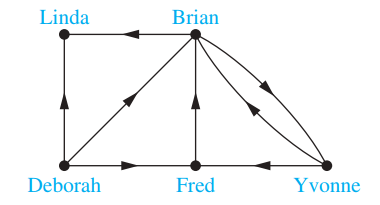
\includegraphics[width=0.4\textwidth]{assets/pic7.png} 
    \caption{Đồ thị ảnh hưởng} % Creates caption underneath graph
\end{figure}


\subsubsection{Mạng kết nối}
Chúng ta có thể lập mô hình các mạng lưới thông tin liên lạc khác nhau bằng cách sử dụng các đỉnh để biểu thị thiết bị và các cạnh để biểu thị loại liên kết truyền thông cụ thể mà ta quan tâm.

\textbf{Ví dụ: Đồ thị cuộc gọi}

Đồ thị có thể được sử dụng để mô hình hóa các cuộc gọi điện thoại được thực hiện trong một mạng lưới, chẳng hạn như mạng điện thoại đường dài. Đặc biệt, một đồ thị có hướng có thể được sử dụng để lập mô hình các cuộc gọi, trong đó mỗi số điện thoại được biểu diễn bằng một đỉnh và mỗi cuộc gọi điện thoại được biểu diễn bằng một cạnh có hướng. Cạnh đại diện cho cuộc gọi bắt đầu từ số điện thoại thực hiện cuộc gọi và kết thúc ở số điện thoại nhận cuộc gọi. Ta cần các cạnh có hướng bởi vì hướng mà cuộc gọi được thực hiện rất quan trọng. Ta cũng cần các cạnh song song có hướng vì cần biểu diễn mỗi cuộc gọi được thực hiện từ một số điện thoại cụ thể đến một số thứ hai.
Một đồ thị cuộc gọi điện thoại nhỏ được hiển thị trong Hình (a), đại diện cho bảy số điện thoại. Ví dụ: Đồ thị này cho thấy ba cuộc gọi đã được thực hiện từ 732-555-1234 đến 732-555-9876 và hai cuộc gọi theo hướng khác, nhưng không có cuộc gọi nào được thực hiện từ 732-555-4444 đến 6 số còn lại ngoại trừ 732-555-0011. Khi chỉ quan tâm đến việc có cuộc gọi nào kết nối hai số điện thoại hay không, ta sử dụng biểu đồ vô hướng với một cạnh kết nối các số điện thoại khi có cuộc gọi giữa các số này. Phiên bản này của đồ thị cuộc gọi được hiển thị trong Hình (b).
Đồ thị cuộc gọi mô hình hóa hoạt động gọi điện thoại trong thực tế có thể rất lớn. Ví dụ, một đồ thị cuộc gọi được nghiên cứu tại Nhà mạng AT-T về các cuộc gọi trong 20 ngày, có khoảng 290 triệu đỉnh và 4 tỷ cạnh.

\begin{figure}[H] % places figure environment here   
    \centering % Centers Graphic
    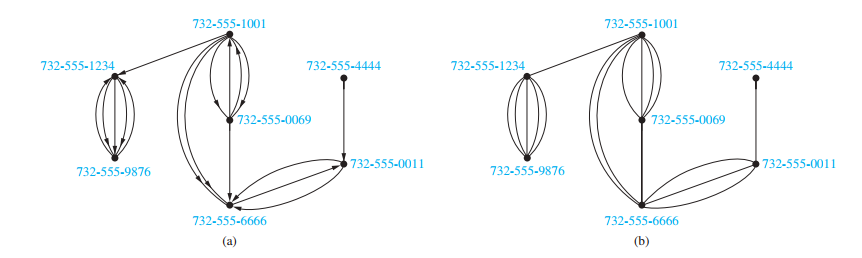
\includegraphics[width=0.8\textwidth]{assets/pic8.png} 
    \caption{Đồ thị cuộc gọi} % Creates caption underneath graph
\end{figure}


\subsubsection{Mạng thông tin}
Đồ thị có thể được sử dụng để mô hình hóa nhiều mạng lưới khác nhau liên kết các loại hình thông tin cụ thể. Trong phần này, ta sẽ mô tả cách lập mô hình web bằng đồ thị. Đồng thời mô tả cách sử dụng biểu đồ để mô hình hóa các trích dẫn trong các loại tài liệu khác nhau.

\textbf{Ví dụ: Đồ thị web}
Trang web có thể được mô hình hóa dưới dạng một đồ thị có hướng, trong đó mỗi trang web được biểu diễn bởi một đỉnh và ở đó một cạnh bắt đầu từ trang web a và kết thúc ở trang web b nếu có một liên kết trên a trỏ đến b. Vì việc tạo mới hoặc xóa các trang web diễn ra hầu như trong mỗi giây, nên biểu đồ web thay đổi gần như liên tục. Nhiều người đang nghiên cứu các thuộc tính của đồ thị web để hiểu rõ hơn về bản chất của web.

\textbf{Ví dụ: Đồ thị trích dẫn}
Đồ thị có thể được sử dụng để thể hiện những trích dẫn trong các loại tài liệu khác nhau, bao gồm các bài báo học thuật, bằng sáng chế và ý kiến pháp lý. Trong các biểu đồ như vậy, mỗi tài liệu được biểu diễn bằng một đỉnh và có một cạnh từ tài liệu này đến tài liệu thứ hai nếu tài liệu đầu tiên trích dẫn tài liệu thứ hai trong danh sách trích dẫn của nó. (Trong một bài báo học thuật, danh sách trích dẫn là thư mục, hoặc danh sách tài liệu tham khảo; trong bằng sáng chế, danh sách các bằng sáng chế trước đó được trích dẫn; và với các ý kiến pháp lý, đó là danh sách các ý kiến trước đó). Một đồ thị trích dẫn là một đồ thị có hướng không có khuyên hoặc cạnh song song.




